\documentclass[a4paper,english,thesis]{dcsbook}

\usepackage{latexsym}
\usepackage[utf8]{inputenc}
\usepackage{graphicx}
\usepackage{hyperref}
\usepackage{amsfonts}
\usepackage{subfig}
\usepackage{appendix}
\usepackage{babel}

\usepackage{multirow}

\usepackage{pstricks}
\usepackage{psfrag}
\usepackage{xcolor}
\usepackage{tikz}
\usetikzlibrary{arrows,chains,decorations.pathmorphing,backgrounds,positioning,fit}

\usepackage{algorithm}
\usepackage{algpseudocode}

\renewcommand{\appendixtocname}{Appendices}
\renewcommand{\appendixpagename}{Appendices}

\author{Igor~Kupczy\'nski}
\university{Pozna\'n University of Technology}
\supervisor{prof. dr hab. inz. Roman~S\l{}owi\'nski}
\date{Pozna\'n 2010}

\title{Interactive Evolutionary Algorithm \\ for Robust Multi-Objective
  Optimization}

\tikzset{redrect/.style={
      % The shape:
      rectangle,
      % The size:
      minimum size=6mm,
      % The border:
      very thick,
      draw=red!50!black!50,         % 50% red and 50% black,
      % and that mixed with 50% white
      % The filling:
      top color=white,              % a shading that is white at the top...
      bottom color=red!50!black!20, % and something else at the bottom
      % Font
      font=\itshape
    }
}

\tikzset{roundrect/.style={
    % The shape:
    rectangle,minimum size=6mm,rounded corners=3mm,
    % The rest
    very thick,draw=black!50,
    top color=white,bottom color=black!20,
    font=\ttfamily
  }
}

\tikzset{greenrect/.style={
      % The shape:
      rectangle,
      % The size:
      minimum size=6mm,
      % The border:
      very thick,
      draw=green!50!black!50,         % 50% red and 50% black,
      % and that mixed with 50% white
      % The filling:
      top color=green!50!black!20,
      bottom color=white,
      % Font
      font=\ttfamily
    }
}


\begin{document}
\maketitle
\frontmatter
\tableofcontents{}
\mainmatter

\chapter{Introduction}
Optimization is a~process of finding the best solution from a~set of available
alternatives. In the simplest case it involves only a~single objective. An
objective is a~problem's goal, whose value has to be maximized (or
minimized). An optimization problem consists of a~set of decision variables;
values of those variables affect the problem's objectives. A~domain of the
problem --- a~set of possible values that can be taken by the decision
variables --- may be subject to additional constraints. An assignment of
values to the decision variables is called a~solution. A~solution is feasible
if the values meet the constraints imposed on the problem. Therefore, the task
of optimization is to find a~feasible solution, which maximizes (minimizes)
the value of the problem's objectives.

Optimization is a~field of applied mathematics, which has gained importance
during and after the Second World War. The driver for developments in the
field are real-life, mainly military or industrial problems. They are often
large-scale and of high importance; solving a~problem of this kind usually
yields a~profit outranking the costs that one has to bear to employ a~formal
approach. To use optimization methods one has to formulate a~problem in a
mathematical way --- build a~model of the problem. Therefore, it is common to
make a~distinction between a~stakeholder --- a~decision maker (DM) having
expert knowledge in a~problem domain and an analyst --- a~mathematician or
a~scientist that will create the model and choose an appropriate optimization
technique.

If there is only one, single objective in the problem definition, then the
optimization usually results in a~one optimal solution which has the best
possible value of the goal. However, this is not the case when multiple goals
are considered. Usually the optimal value for one goal is far from being an
optimal for the other; for example, consider a~simple problem of choosing a
laptop computer to buy --- the one with the highest performance is not the
cheapest and the cheapest will probably not offer a~state-of-the-art
performance. No trade-offs between objectives can be assumed \textit{a
  priori}. This is because the importance of each goal may be different for
different decision makers --- someone can choose a~cheap computer, while the
other will opt for the highest performance available. However, one can
indicate a~non-dominated set of solutions --- the Pareto-frontier of the
problem. Informally, a~solution is Pareto-efficient if a~value of any of its
criteria can not be improved without worsening the other values. In the laptop
example it could be a~list of the cheapest computers for different
performances.

Multi-Objective Optimization (MOO) methods are usually sophisticated, with
many parameters for the analyst to fine-tune them. However, the decision maker
is usually not interested in the details of the method, but only in a~single
recommendation, possibly along with a~justification. The analyst will set up
the method and its parameters based on his or her intuition and on a~research
carried out earlier. An experienced analyst can usually decide what
parameters' values should be used, but still it may be impossible to set the
values precisely to the best possible options. If one can change parameters a
bit and the resulting solution is similar to the one acquired before, then the
solution is called robust. The same applies if the problem model can not be
formulated precisely --- for example, it contains a~value that may be only
estimated, like the future price of a~raw material. The solution should be
resistant to small fluctuations in the problem's model parameters. The
robustness in MOO context is the ability to withstand changes in the
parameters and in the problem formulation; it is a~very important quality of
any MOO technique.

To give final recommendation instead of the Pareto-frontier one has to engage
the decision maker in the process. The method has to be interactive in order
to gather the DM's preferences. It can be done by showing exemplary feasible
solutions and asking the decision maker to rank them or simply by asking about
the inter-criteria trade-offs. These preferences are used to guide the search
of the solution space in the directions desired by the DM. An optimization
technique involving interaction with the decision maker is called the
interactive multi-objective optimization (IMO) technique.

The algorithm is a~well-defined list of instructions for completing a
task. Several researchers suggested that principles of the evolution ---
particularly, the concept of population and survival of the fittest
individuals can be a~good model of operation for multi-criteria optimization
algorithms. Methods using these principles are called the evolutionary
algorithms (EAs) while the whole field of research is the evolutionary
multi-objective optimization (EMO).

In this paper the author presents the DARWIN method. DARWIN is an acronym for
Dominance-based rough set Approach to handling Robust Winning solutions in
INteractive multi-objective optimization. DARWIN is an algorithm proposed by
Salvatore Greco, Benedetto Matarazzo and Roman Słowiński; dedicated for
solving multi-objective optimization problems. It interacts with the decision
maker in order to infer his or her preferences. The preferences are then
stored in the form of decision rules guiding the optimization process. An
evolutionary algorithm is used as an engine for optimization. Therefore DARWIN
combines IMO and EMO paradigms. It allows an analyst to model uncertainty in
the problem definition, thus generating robust solutions.

The thesis consists of six chapters. Firstly, the theoretical background is
presented. A~more detailed description of the DARWIN algorithm follows in the
chapter~\ref{darwin-the-idea}. The chapter~\ref{darwin-implementation}
discusses an implementation on an IBM-PC class computer. Experiment results
are shown and discussed in the chapter~\ref{exp-results}. Finally, areas of
further research are indicated along with conclusions and recommendations
about the method.

\chapter{Multi-Objective Optimization}
Often a~model of a~problem contains multiple objectives. This is the case when
conflicting goals cannot be easily converted to a~single objective. The
decision support when more than one goal is considered to be not an easy task
to perform, however, several approaches exists. These approches are described
in the chapter.

\section{Interactive Approaches to MOO}
\label{sec_ia_in_moo}

The Multi-Objectie Optimization problems usually have multiple Pareto-optimal
solutions. However, the Decision Maker is usually interested in a~single
recommendation --- the single solution he or she may implement. The
most-preferred solution is a solution from the Pareto-frontier of the problem,
for which the DM is convinced it is his or her best option.

To find the most preferred solution, an interaction with the DM is
necessary. A~problem solver needs to know the Decision Maker's preferences in
order to differentiate Pareto-optimal solutions. Without the preferences all
solutions on the Pareto-frontier have to be considered equal.

The DM can build his or her global preference model before an algorithm
solving the problem starts and give this model as an input. This is call the
\textit{a priori} method. However, this method has its weaknesses. It may be
hard for the Decision Maker to give the full preference structure. It is
possible also, that he or she will change his or her preferences after
evaluating solutions received from the problem-solver. 

The interactive approach overcome this weaknesses by involving the DM in the
process. A~basic structure of the approach is shown in
Figure~\ref{imoprocess_uml}. At first, an initial set of solutions is
generated. It can be a subset of the Pareto-frontier or just a set of feasible
solutions. Then, based on the solutions, the Decision Maker specifies his or
her preferences. It can be done by a systematic dialog, asking a series of
questions or asking the DM to indicate ``good'' solutions among the set.

\begin{figure}
  \centering 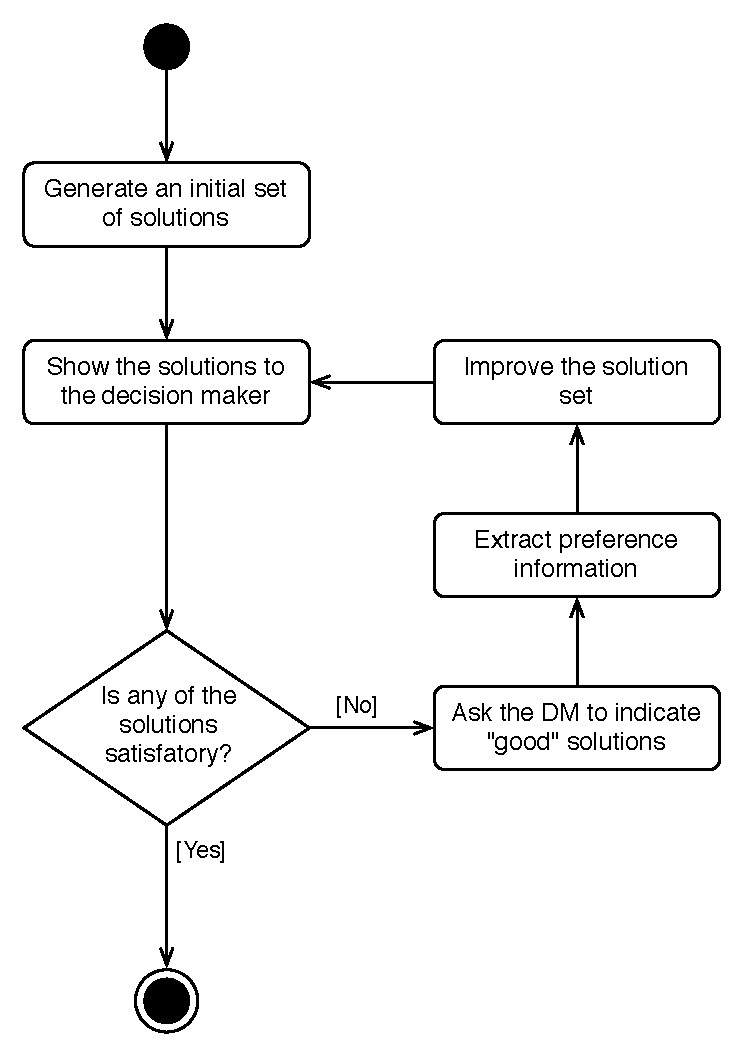
\includegraphics[scale=0.65]{img/imoprocess_uml}
  \caption{An activity diagram for a typical interactive process}
  \label{imoprocess_uml}
\end{figure}

From the DM's answers a preference model is built. This additional preference
information guides the search towards a~region indicated by the Decision
Maker. This can save the computational cost, because the algorithm doesn't
have to go through the whole search space.

Again, new solutions, probably better fitted to the DM's preferences are
generated and the algorithm shows them to him or her. If he or she finds it
satisfactory (or a~stop condition is met) then the algorithm stops. Otherwise
it advances to the next iteration.

There are several types of the IMO methods (consult~\cite{MRW08} for an
in-depth description):
\begin{itemize}
\item \textbf{Trade-off based methods}. A~trade-off is an exchange, a price that
  one is willing to pay (in form of lost on some of the criteria), in order to
  benefit on another criterion (or criteria). These methods ask the DM
  questions about the trade-offs he or she can accept and then, a~preference
  model is inferred based on the tread-offs.
\item \textbf{Reference point approaches} --- the DM specifies bounds on
  values of the objective functions (i.e. reference points) and then, he or
  she can observe the effect of the bounds on the generated solutions.
\item \textbf{Classification-based methods}. It is not possible to improve a
  value of a goal of a solution from the Pareto-frontier without worsening
  other goals of the solutions. In the classification-based methods the DM is
  asked to select goals that can be impaired and the ones that he or she wants
  to improve.
\end{itemize}

The interactive approach requires the Decision Maker's collaboration during
the process, however the approach offers strong benefits to justify this
dedication. Clearly, the computational cost required is lower than in other
approaches, because there is no need to evaluate whole solution space, just
its small subset. The DM may not be able to express a~global structure of his
or her preferences up front. It is also possible that his or her preferences
will change along with the change in understanding of the problem. During the
interactive process the DM has an immediate feedback --- he or she may see how
the decisions are affecting problem solutions.

One can say that solving a Multi-Objective Optimization problem is a
constrictive process, where the Decision Maker learns more about the problem
--- what kind of solutions are possible and how his of her choices influences
the results (see~\cite{MRW08}). As a result, not only the most preferred
solution is given, but also the problem understanding by the DM is better.


\section{Evolutionary Approaches to MOO}
\label{sec_ea_in_moo}

\begin{figure}
  \centering 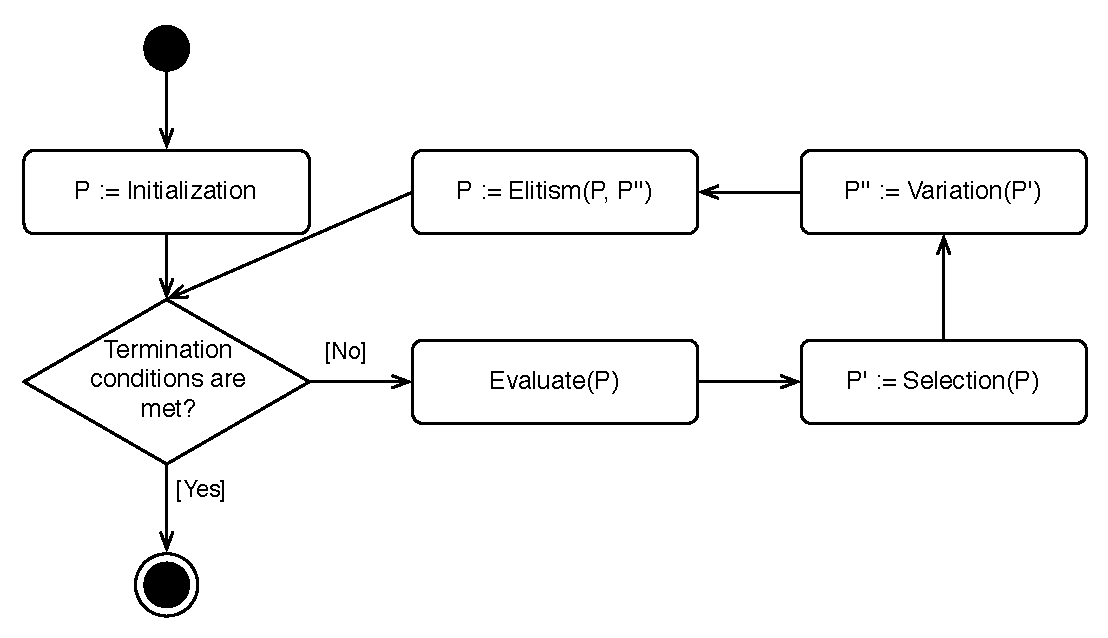
\includegraphics[scale=0.65]{img/eo}
  \caption{An evolutionary optimization procedure}
  \label{eo}
\end{figure}

In 1859, Charles Darwin published his work ``On the origin of
species''~\cite{Dar1859}. He introduced a~scientific theory describing the
evolution of species through the process called natural selection.  According
to the theory, a trait can become less or more common in the population in
dependence on its effect upon the survival and reproduction of the individuals
bearing the trait.

This idea can be easily transfered to the optimization field. A~solution to
a~problem --- that is, the set of values of problem's decision variables ---
is a~single individual in the population. The problem is the environment ---
the higher the solution evaluation on a~given problem, the better it is fitted
to the environment. A~better fitness means higher chance that the traits of
a~solution will be present in the next iteration (an analogue of
a~reproduction success rate). First successful applications of the idea were
done in the electrical engineering field (see~\cite{Fog64}) and in the fluid
mechanics (see~\cite{Rec65, Sch65}).

The main differences between the classical and the evolutionary optimization
(EO) are (see~\cite{Deb08}):

\begin{itemize}
\item \textbf{Population-based}. An EO procedure uses a~population of
  solutions (a~population approach), whereas the classical algorithms maintain
  one solution at a~time (a~point approach). It enables an algorithm to
  maintain multiple optimal solutions, possibly from different parts of the
  solution space. Unfortunately it rises the memory and computational
  footprint of an EO algorithm.
\item \textbf{Stochastic operators}. An EO procedure uses stochastic operators
  (e.g. selection, crossover or mutation) instead of deterministic ones.
\item \textbf{Gradient information}. An EO procedure does not usually use
  gradient information directly in performing a~search. This means that the
  procedure is immune to local optima in a~search space. However, the EO
  procedure may not be competitive with dedicated gradient approach.
\end{itemize}

The basic evolutionary optimization procedure is shown in Figure~\ref{eo}. The
algorithm starts with creating a~population of solutions. Usually the
population is created at random within bounds of decision variables. Then
a~succesion of generations starts. The populations is updated by a~sequence of
operators.

First, the population is evaluated. The evaluation means establishing an
relative preference order, that is sorting solutions from the best to the
worst. After the evaluation the algorithm chooses solutions to fill the mating
pool. The better the solution the higher the probability to be chosen. Then,
the variation operator is being used. It is a series of steps, such as
crossover or mutation, generating a~succeeding generation (an offspring) from
parents in the mating pool. The crossover ensures that parents' traits will be
present in the next generation while the mutation acts as local search in the
solution's neighborhood. Finally, the elitism operator combines the old
population with the newly created offspring. Coping best solutions from the
former ensures the algorithm has a monotonically non-degrading value of the
best solution.

\begin{figure}
  \centering 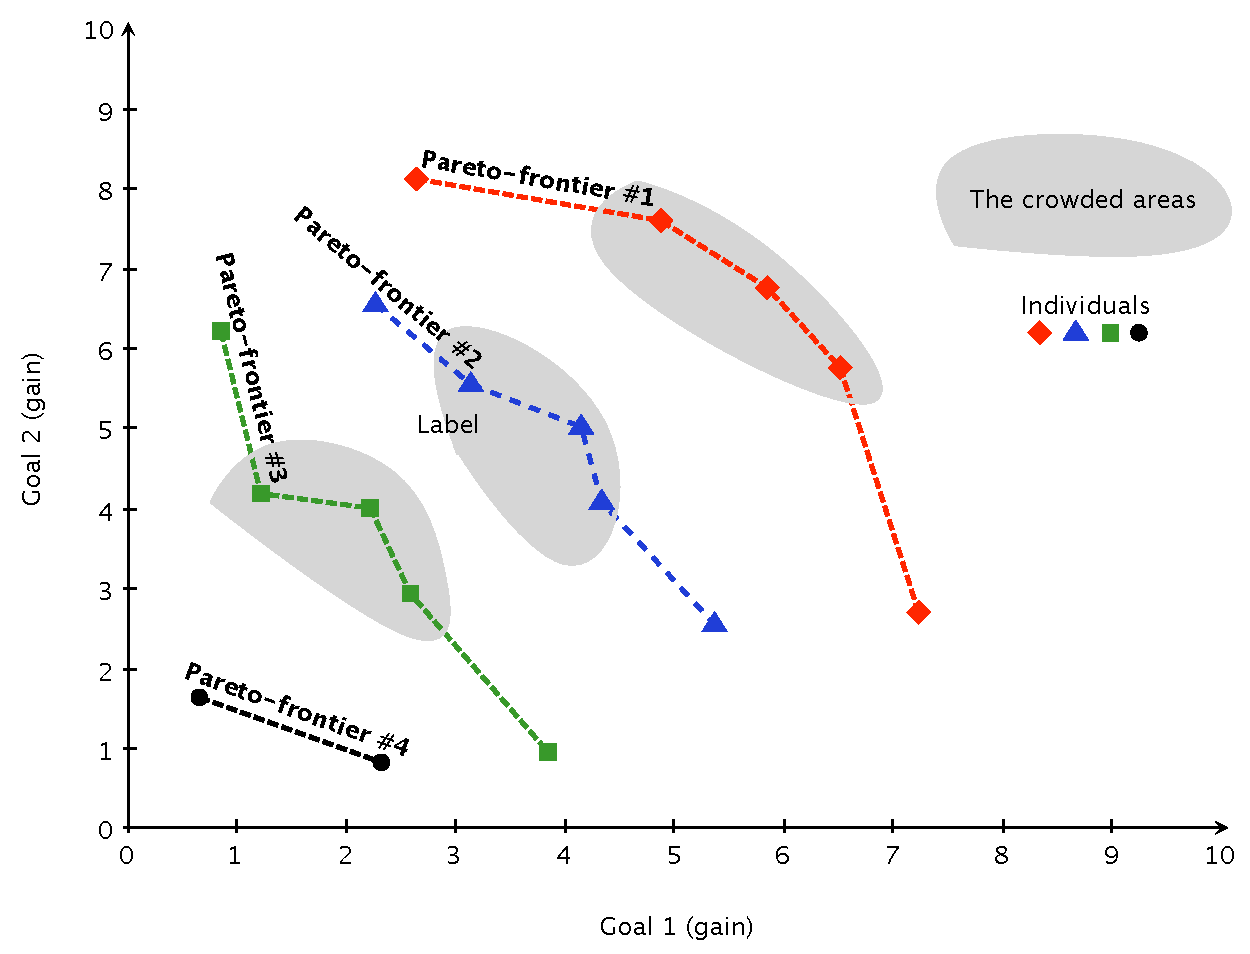
\includegraphics[scale=0.55]{img/nsga}
  \caption{The NSGA-II evaluation}
  \label{nsga}
\end{figure}

The choice of a~fitness function is critical to the algorithm's
performance. In case of a~problem with a~single criterion this is trivial ---
a~value of the goal can be used. However, in the case of the Multi-Objective
Optimization, there are a number of objective functions to be
optimized. A~possible approach to the problem is to use the dominance
principle (\cite{Gol89}):

\vspace{0.5cm} \textit{A solution x is said to dominate the other solution y,
  if both of the following conditions are true:}
\begin{enumerate}
\item \textit{The solution x is no worse than y in all objectives. Thus, the
    solutions are compared based on their objective function values.}
\item \textit{The solution x is strictly better than y in at least one
    objective.}
\end{enumerate}

All the solutions that are non-dominated by any other solution are forming the
Pareto-frontier of the problem.

According to~\cite{Deb08} there are two ideal goals of the EMO:
\begin{enumerate}
\item Find a set of solutions which lies on the Pareto-optimal front, and
\item Fina a set of solutions which is diverse enough to represent the entire
  range of the Pareto-optimal front.
\end{enumerate}

An example of the Evolutionary Multi-objective Optimization (EMO) algorithm is
the NSGA-II (\cite{Deb00}). The basic idea behind the algorithm is to assign
each solution in a~population to a~number of different Pareto-frontiers. All
non-dominated individuals are assigned to first Pareto-frontier and then
removed from the population. All non-dominated individuals after the removal
are then assigned to second frontier. The process repeats until there are
individuals in the population. The lower the number of the~frontier, which an
individual belongs to, the higher the fitness function for it. In case of draw
the crowding score this taken into account --- the lesser the crowd in the
solution's neighborhood in an objective space, the better the solution's
evaluation. This is illustrated in fig.~\ref{nsga}.


\section{Dominance-Based Rough Set Approach to MOO}
\label{sec_drsa_in_moo}

A rough set is an approximation of a~conventional set --- a pair of sets being
a~lower and an upper approximation of the original set (\cite{Paw82}). The
lower approximation is a~set of all objects that unambiguously can be
classified as members of the target set. On the other hand, the upper
approximation is a~set containing objects that cannot be unambiguously
classified as members of the complement of the target set.  A~boundary region
is the part of solution space being part of the upper approximation, but not
the lower one.

\begin{figure}
  \centering 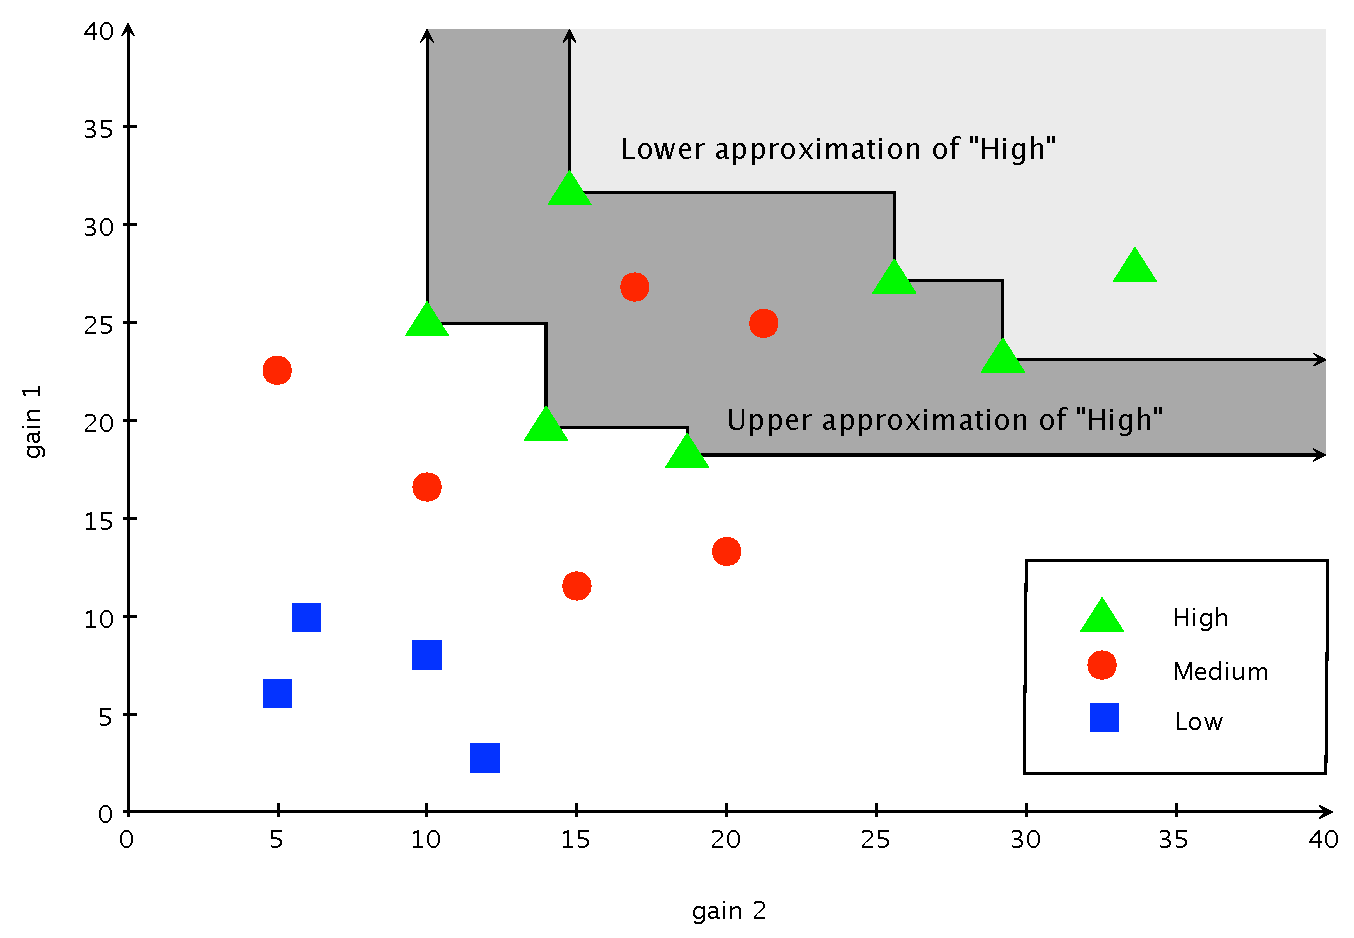
\includegraphics[scale=0.5]{img/drsa}
  \caption{An example of the DRSA approach}
  \label{drsa}
\end{figure}

Dominance-based Rough Set Approach (DRSA) is an extension of the rough set
theory introduced in~\cite{GMS01, GMS02, GMS05}. The indiscernibility relation
is replaced by the dominance relation (defined in the former section). DRSA is
applicable in the decision support field.

DRSA can model the situations in which there are objects --- vectors of values
in the decision variable space --- and each object belongs to one of the
decision classes. The classes are sorted in a~preference order. An example is
shown in Figure~\ref{drsa}.

The data in Dominance-based Rough Set Approach are often presented in
a~decision table. The objects being considered are written in table rows, the
decision attributes are table columns. The last column is classification of
the objects to a decision classes. A formal definition of the decision table
can be easily found in the literature. An example is given in
Table~\ref{t:dec_tab-example}.

\begin{table}
  \centering
  \begin{tabular}{c c c c | c}
   \hline
   Student & Mathematics & Physics & Literature & Overall class \\
   \hline
   \hline
   1 & good & medium & bad & bad \\
   2 & medium & medium & bad & medium \\
   3 & medium & medium & medium & medium \\
   4 & medium & medium & medium & good \\
   5 & good & medium & good & good \\
   6 & good & good & good & good \\
   7 & bad & medium & medium & bad \\
   8 & bad & bad & medium & bad \\
   \hline
  \end{tabular}
  \caption{An example of the decision table}
  \label{t:dec_tab-example}
\end{table}

On the basis of the table, decision rules may be induced. They are generalized
description of the knowledge represented in the table. A~decision rule is a
Horn clause (see~\cite{Hor51}) in form of \textit{``if~..., then~...''}. The
former part is called \textit{condition} and the latter ---
\textit{consequent}. The condition part compares a~value of an object
attributes with given thresholds and the consequent part represents the object
classification if the condition part holds. Rules can be either
\textit{certain} --- based on objects from the lower approximation of the
class, \textit{possible} --- based on objects from the upper approximation and
\textit{approximate} --- based on the boundary region. Each decision rule
should be minimal, i.e. cardinality of the set of conditions should be
minimal.

Example rules generated from Table~\ref{t:dec_tab-example}:
\begin{enumerate}
\item If \textit{Literature $\ge$ good} then \textit{Student $\ge$ good},
\item If \textit{Mathematics $\le$ bad} and \textit{Physic $\le$ medium} then
  \textit{Student $\le$ bad},
\item If \textit{Mathematics $\ge$ medium} then \textit{Student $\ge$ medium}
  (possible).
\end{enumerate}

DRSA can handle uncertainty and contradictions in the data, thus it can model
a~wide class of problems. For each rule $r$ given in from $\Phi \to \Psi$
following measures are defined:
\begin{itemize}
\item Support: $\textit{supp}(\Phi, \Psi) = \textit{cardinality}(||\Phi \land
  \Psi||)$ --- is the number of objects for which the condition of the rule
  holds and the object classification is consistent with the consequent of the
  rule.
\item Confidence: $\textit{confidence}(\Phi, \Psi) =
  \dfrac{\textit{supp}(\Phi, \Psi)}{\textit{cardinality}(||\Phi||)}$ --- is
  the number of objects supporting the rule in a~relation to the number of
  objects for which the rule's condition holds.
\end{itemize}.

Objects supporting rule$_3$ are \{S2, S3, S4, S5\}, but the condition part
holds also for S1. The support is: $\textit{supp}(r_3) = \frac{4}{5} = 0.8$.

To extract all rules from the decision table one can use the All Rules
algoritm (an optimized version is described in~\cite{Zur01}). The other option
is to use the DomLem algorithm (\cite{GMS+01}) generating minimal set of rules
covering all the objects from a given table.


%%% Local Variables: 
%%% mode: latex
%%% TeX-master: "main"
%%% End: 


\chapter{DARWIN, the Idea behind the Method}
\label{darwin-the-idea}
The basic idea of Darwin method was introduced in~ \cite{GMS09}. This idea will
be described in the following paragraph.

\section{Background}

The method combines two different approaches --- Interactive Multi-Objective
Optimization (IMO, see~[inref]) and Evolutionary Multi-Objective Optimization
(EMO, see~[inref]).

In the IMO paradigm one wants to elicit decision maker's preferences by
involving him or her in the process. This is done by a systematic dialog with
the decision maker (the DM). Questions are being asked and the DM provides
answers. Preference information is extracted on the basis of these answers. Algorithm
can then use the knowledge to produce solutions better fitted to his or her
preferences. The IMO framework is presented in
fig.~\ref{fig:interactive-process}.

\begin{figure} 
  \begin{center}
    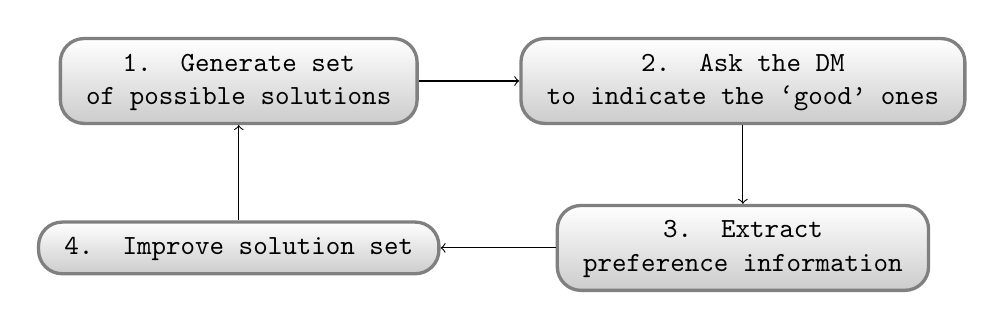
\begin{tikzpicture}
      \matrix[row sep=10mm, column sep=10mm]{

        
        \node (gen)     [roundrect] {
          \begin{tabular}{c}
            1. Generate set\\
            of possible solutions
        \end{tabular}}; &

        \node (ask) [roundrect] {
          \begin{tabular}{c}
            2. Ask the DM \\
            to indicate the `good' ones
        \end{tabular}}; \\

        \node (use) [roundrect] {
          \begin{tabular}{c}
            4. Improve solution set
        \end{tabular}}; &

        \node (store) [roundrect] {
          \begin{tabular}{c}
            3. Extract \\
            preference information
        \end{tabular}}; \\
      };
      \path (gen) edge[->] (ask);
      \path (ask) edge[->] (store);
      \path (store) edge[->] (use);
      \path (use) edge[->] (gen);
    \end{tikzpicture}
    \caption{Typical Interactive Multiobjective
      Optimization process framework\label{fig:interactive-process}}
  \end{center} 
\end{figure} 

The rationale behind the interactive process is that the decision maker is
interested only in a small subset of preferred solutions or even in a single
most preferred one.

This process makes it possible to gather preference information and then use
this information to construct better solutions. However, this is just a
framework, so details are left up to the analyst. One has to think
particularly how to extract and store knowledge gathered on DM's answers and
how to use this knowledge to generate and provide solutions better fitted to
decision maker's preferences.

Human factor is yet another thing to consider. The DM is a human being and
thus his or her behavior is constantly changing. The challenge here is to find
out what questions should be asked and how often, as well as how many
intermediate solutions should be presented to evaluate.

DARWIN is a realisation of the IMO process. It keeps generating solutions and
improving them on the basis of DM's feedback. It only asks the DM to mark
potentially good solutions, so that only problem-domain knowledge is required;
its user does not need to have expert knowledge in the decision support field.

Evolutionary Multi-Objective Optimization (EMO) provides a computational
engine for generating new, better solutions from existing ones --- better in
sense of objective function defined in the solution space. Most of the EMO
methods are approximating Pareto-optimal front by a set of solutions. So one
solution is better than the other if the former Pareto-dominates the
latter. In case of two equivalent ones another factors have to be taken into
account (for example crowding score in NSGA2 [ref]). This is the case because
if no preference information is given all Pareto-optimal solutions have to be
considered equivalent.

It seems natural to combine these two described approaches --- Interactive
Multi-Objective Optimization and Evolutionary Multi-Objective
Optimization. (TODO: maybe a note and a ref about combining these two
approaches). IMO is just a process framework but still needs an engine to
generate and improve solutions. EMO is such an engine. On the other hand for
EMO involving the decision maker in the procedure results in gathering
preference information. This information allows the procedure to focus on a
specific region of Pareto-front --- the most relevant one to the decision
maker. In this way IMO and EMO are complementing each other.

\begin{figure}
  \centering 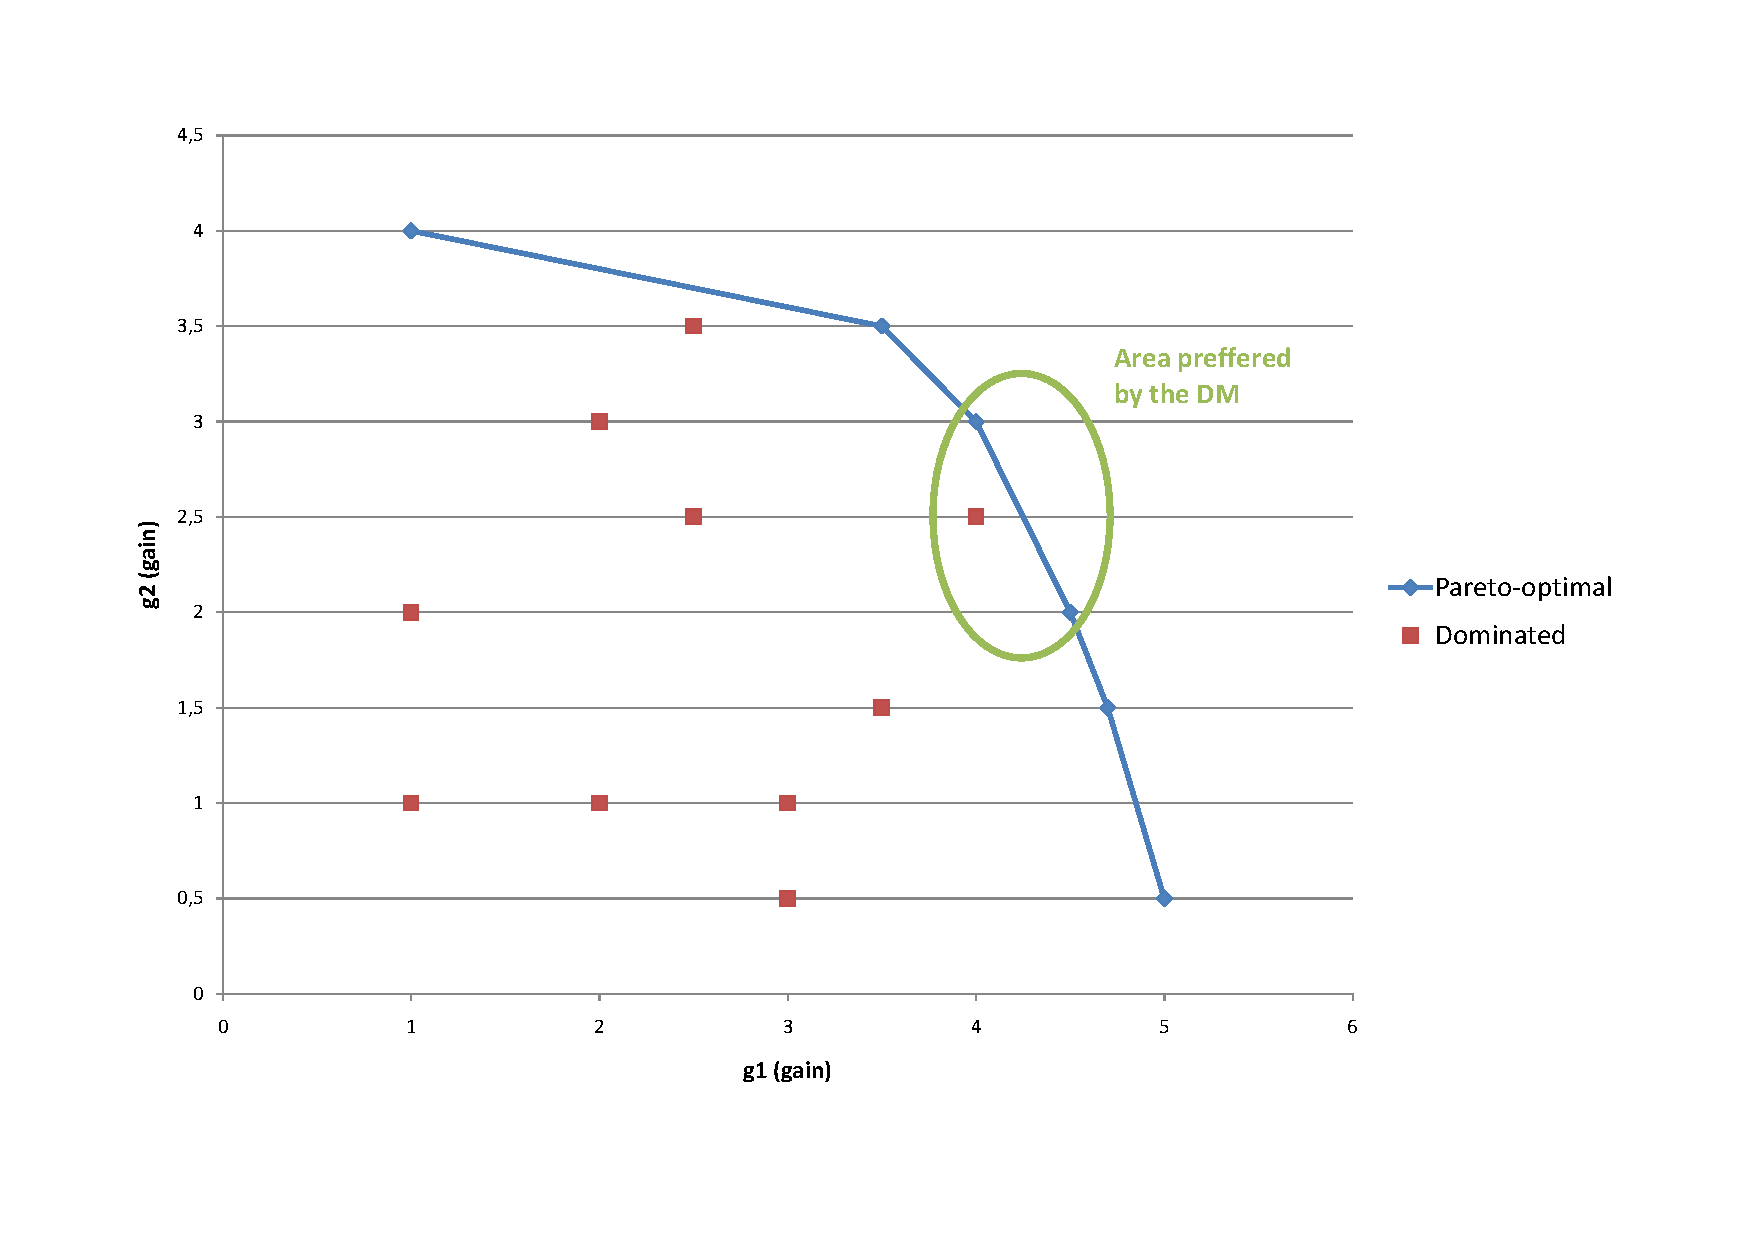
\includegraphics[width=1.2\textwidth]{img/pareto}
  \caption{Pareto-front and area preferred by the decision maker}
  \label{pareto}
\end{figure}

This is important because of the ``human factor''. If the number of solutions
becomes huge, the DM can not effectively analyze them and find the one that
fits his/her preferences best, thus Pareto-optimality is not sufficiently
discriminative. However, guiding the search to preferred regions of the
solution space allows the method to converge faster to good solutions. It is
shown in fig.~\ref{pareto}.

DARWIN uses EMO procedure to improve generated solutions based on the DM's
preferences.


\section{Modeling of uncertainty}

It is often the case that not all numbers and coefficients are precisely
known. It may be easier for the decision maker to formulate the
Multi-Objective Optimization problem giving the problem coefficients in the
form of intervals of possible values. For example, instead of saying that
product price will equal 20 units one can say it will be in the $[19, 21]$
interval. In this situation the decision maker is often interested in finding
the best robust solution --- that is good and possible in a large part of
uncertainty scenarios. DARWIN allows to give the coefficients in a form of
intervals.

\begin{figure}
  \centering 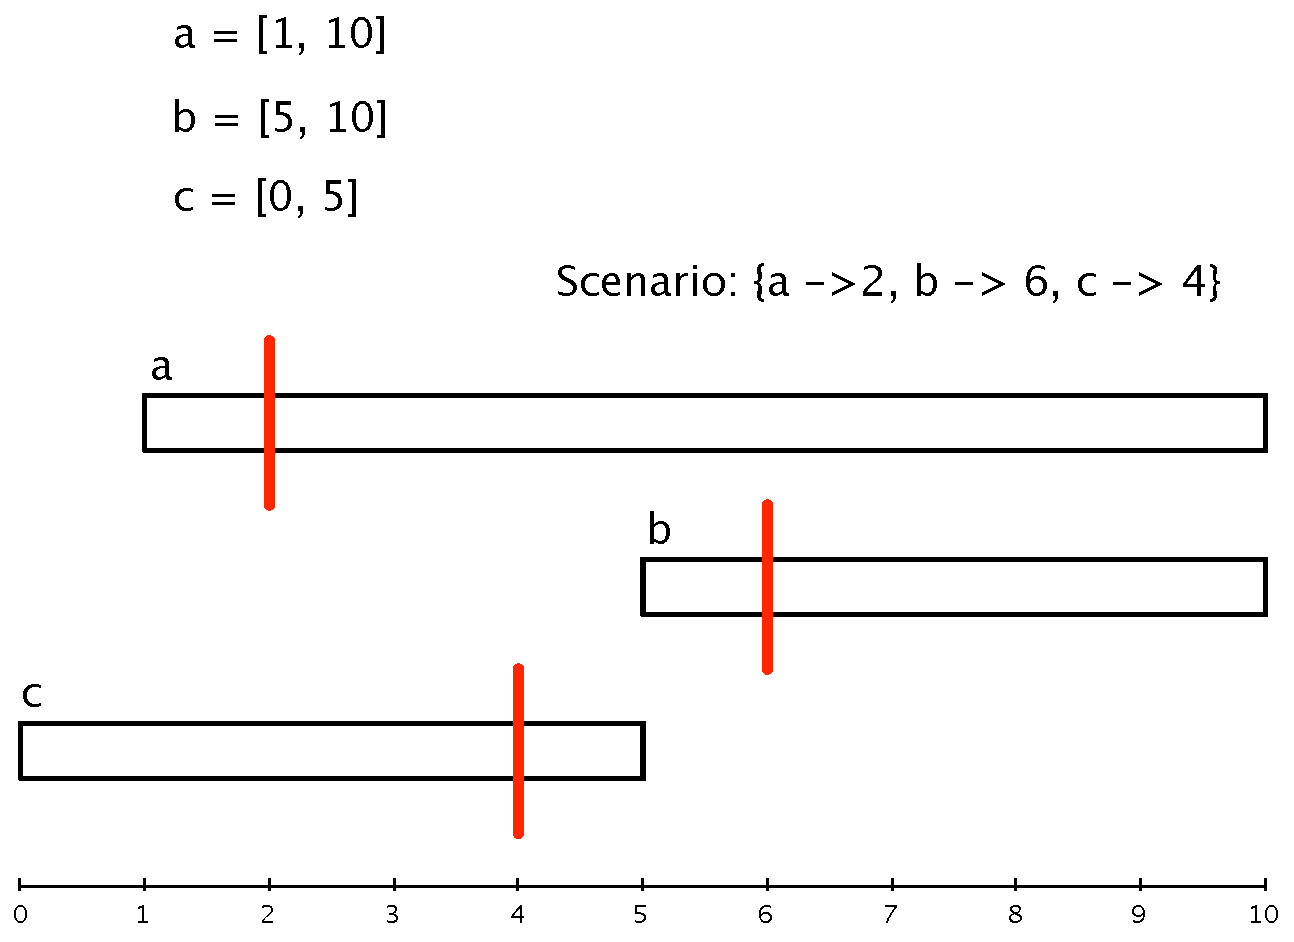
\includegraphics[width=0.5\textwidth]{img/scenario}
  \caption{Scenario --- set of intervals fixed on specific values}
  \label{scenario}
\end{figure}

The set of all of the problem's coefficients given as intervals and fixed on
one of possible values will be called scenario of imprecision (see
fig.~\ref{scenario}). If intervals are allowed, it is impossible to calculate
the exact value of problem's objectives for given solutions. To handle this
case all the considered solutions are evaluated over a~set of uncertainty
scenarios.

\begin{figure}
  \centering 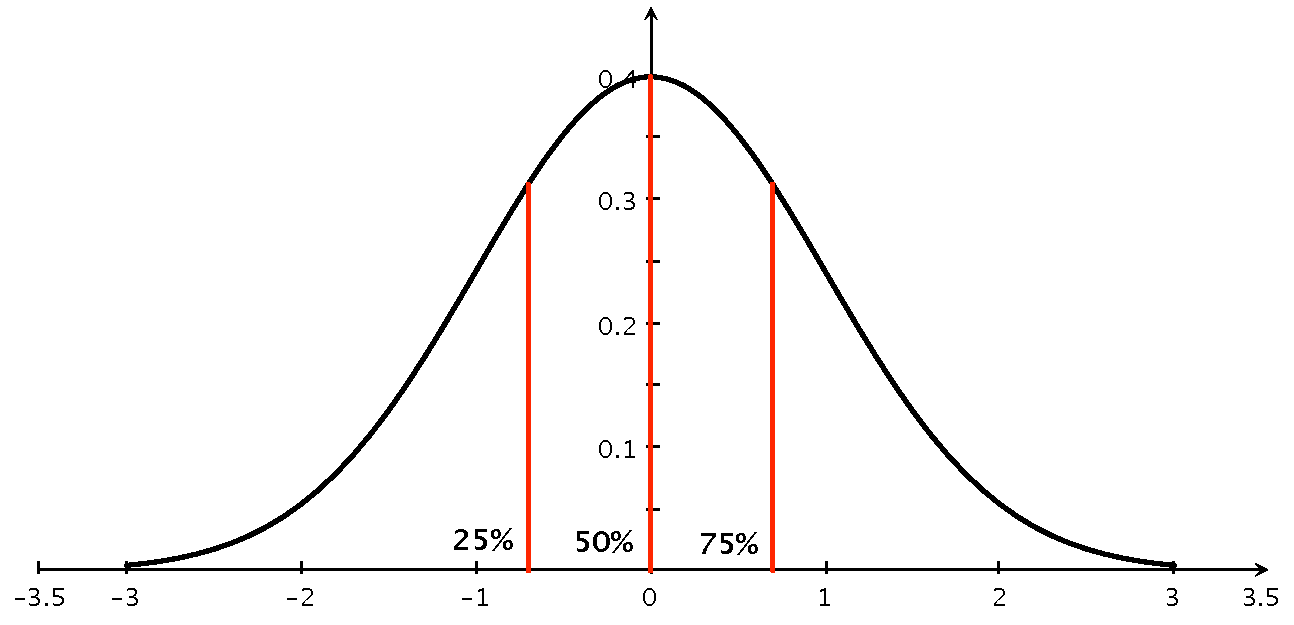
\includegraphics[width=0.8\textwidth]{img/percentile}
  \caption{Percentiles of the normal distribution}
  \label{percentiles}
\end{figure}

 Results of this evaluation are then aggregated to quantile space. The
 quantiles are points taken at regular intervals from the cumulative
 distribution of a random variable. If the interval consists of $0.01$ of the
 distribution, then the quantiles are called percentiles (percentiles of the
 normal distribution are shown in fig.~\ref{percentiles}). Instead of
 presenting all of the results, the method calculates meaningful quantiles of
 results distribution for each objective. For example, percentiles (like $1\%,
 25\%$ and $50\%$) can be chosen. Percentiles divide ordered data into 100 of
 equally-sized subsets --- $1\%$ percentile is the best of $1\%$ worst
 solutions or alternatively the worst of $99\%$ of the best solutions.

Choice of these quantiles is connected with the DM's attitude towards risk. If
he or she wants to avoid risk then his/her decision will be focused on
quantiles from the beginning of the distribution (e.g. $10\%$). On the other
hand, when he or she is interested in the best possible solution even if there
is a risk involved, then the quantiles from the end of the distribution will
be inspected (e.g. $75\%$).

In DARWIN the DM's preferences are gathered and stored using DRSA methodology
(see~[inref]). Dominance-Based Rough Set Approach is a~framework for reasoning
about partially inconsistent preference data. DRSA already has successful
applications in IMO area ([ref]).

DRSA will be applied in IMO process. After selecting ``good'' solutions from
the provided set the decision rules are induced to store the
preferences. These rules are given in the form of \textit{``If ... then
  ...''}. Conditional part is a disjunction of conditions on attributes from
quantile space. These attributes are compared to specific values, e.g.
$\text{profit}_{25\%} >= 100 \land \text{time}_{1\%} <= 10$. The consequent
part assigns a solution to a class (\textit{at least} or \textit{at most}),
e.g. Class \textit{at least} Good. So the whole rule would be If
$\text{profit}_{25\%} >= 100 \land \text{time}_{1\%} <= 10$ then Class
\textit{at least} Good.

\section{The algorithm}

DARWIN can operate on Multi-Objective Optimization (MOO) problems defined as
follows:

\begin{equation}
[ f_1(x), f_2(x), \dots, f_k(x) ] \rightarrow  \max
\end{equation}
subject to:
\begin{equation}
\begin{array}{l}
g_1(x) \geq b_1 \\
g_2(x) \geq b_2 \\
\dots \\
g_m(x) \geq b_m
\end{array}
\end{equation}

Where:
\begin{description}
\item $x = [x_1, x_2, \dots, x_n]$ is a vector of decision variables, called a
  solution;
\item $f_1(x), f_2(x), \dots, f_k(x)$ are objective functions,
  $f: x \rightarrow \mathbb{R}$;
\item $g_1(x), g_2(x), \dots, g_m(x)$ are constraint functions,
  $f: x \rightarrow \mathbb{R}$;
\item $b_1, b_2, \dots, b_m$ are real-valued right hand sides of the
  constraints.
\end{description}

It is possible to give some of the coefficients in objective functions or
constraints in the form of intervals (thus modeling ignorance --- uncertainty
about real value of a coefficient). A vector of fixed values for each interval
is called \textit{scenario} of imprecision (see fig.~\ref{scenario}).

DARWIN is composed of two nested loops --- exterior and interior. The former
is a realisation of an interactive process and the latter is an EMO engine
dedicated to improve solutions based on the decision maker's preferences. This
is illustrated in fig.~\ref{fig:darwin-ext}.

\begin{figure} 
  \begin{center}
    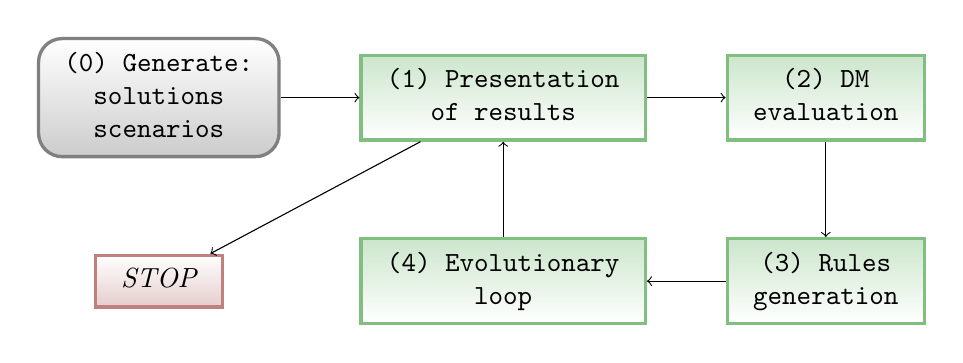
\begin{tikzpicture}
      \matrix[row sep=10mm, column sep=10mm]{

        
        \node (gen)     [roundrect] {
          \begin{tabular}{c}
            (0) Generate:\\
            * solutions\\
            * scenarios
        \end{tabular}}; &

        \node (presentation) [greenrect] {
          \begin{tabular}{c}
            (1) Presentation \\
            of results
        \end{tabular}}; &

        \node (eval) [greenrect] {
          \begin{tabular}{c}
            (2) DM\\
            evaluation
        \end{tabular}}; \\

        \node (stop) [redrect] {
          \begin{tabular}{c}
            STOP
        \end{tabular}}; &

        \node (inner) [greenrect] {
          \begin{tabular}{c}
            (4) Evolutionary \\
            loop
        \end{tabular}}; &

        \node (rules) [greenrect] {
          \begin{tabular}{c}
            (3) Rules \\
            generation
        \end{tabular}}; \\
      };
      \path (gen) edge[->] (presentation);
      \path (presentation) edge[->] (eval);
      \path (eval) edge[->] (rules);
      \path (rules) edge[->] (inner);
      \path (inner) edge[->] (presentation);
      \path (presentation) edge[->] (stop);
    \end{tikzpicture}
    \caption{DARWIN states and transitions. Steps (1) - (4) are forming
      exterior loop and step (4) is the interior loop.\label{fig:darwin-ext}}
  \end{center} 
\end{figure}

\begin{algorithm}
\caption{DARWIN's exterior loop}\label{alg:extloop}
  \begin{algorithmic}[1]
    \State $X \gets$ \Call{GenerateSolutions}{} \label{algin:solgen}
    \State $S \gets$ \Call{GenerateScenarios}{} \label{algin:scengen}
    \Loop
    \ForAll{$x \in X, s \in S$} \label{algin:evstart} \Comment{Evaluate each
      solution over all of the scenarios}
    \State \Call{Evaluate}{$x, s$} 
    \EndFor{} \label{algin:evstop}
    \State $\text{isSatisfied} \gets$ \Call{PresentResults}{} \label{algin:dmshow}
    \If{$\text{isSatisfied}$}
    \State \textbf{stop}$\qed$ 
    \Else
    \State $X \gets$ \Call{AskToMarkGood}{$X$} \label{algin:dmmark}
    \EndIf
    \State rules $\gets$ \Call{InduceDecisionRules}{$X$} \label{algin:rules}
    \State $X \gets$ \Call{EmoProcedure}{rules} \Comment{the interior loop} \label{algin:intloop}
    \EndLoop{}
  \end{algorithmic}
\end{algorithm}


The exterior loop algorithm, corresponding to the IMO interactive process is
shown on alg.~\ref{alg:extloop}. A More detailed description of each step
follows.

First, one has to generate a set of feasible solutions to the MOO problem
first. This can be done using the Monte Carlo method. The Monte Carlo concept
itself is not new. A~concept of statistical sampling became popular after
digital computing machines had been invented (see~[ref]). This method can be
described as random sampling a domain of a problem. In the most basic variant
one can just pick a solution at random and check if it is
feasible. Unfortunately, it will be impossible unless the non-feasible space
is only a small part of the domain. Additional hints for the generator, for
example in the form of analyst's suggestions, can be taken into account.

At this stage goals and constraints are allowed to contain intervals
corresponding to the uncertainty of a model. Thus a set of scenarios needs to
be generated. Each of these scenarios is a realisation of the problem with
fixed values of the intervals (see~[inref]). It is worth noting that if the
problem constraints are given in an uncertain form --- that is containing
coefficients in the form of intervals --- it could be impossible to determine
whether a given solution is possible. If that is the case, then lines
\ref{algin:solgen} and \ref{algin:scengen} should be swapped and feasibility
of a solution set should be checked on generated scenarios.

In lines \ref{algin:evstart} to \ref{algin:evstop} each solution if evaluated
over each scenario. Results of this evaluation phase are then gathered and
presented to the decision maker in \ref{algin:dmshow}. The DM is a human being
though, so in order to get valuable feedback one need to show the data in
aggregated form. The authors proposed a meaningful quantiles to be presented
(see~[inref]). For example $f^{1\%}_1(x), f^{25\%}_1(x), f^{50\%}_1(x),$
$\dots, f^{1\%}_k(x), f^{25\%}_k(x), f^{50\%}_k(x)$ for all $x \in X$.

If the DM finds solution in the set of presented ones satisfactorily, then the
problem is solved and algorithm ends here. If not, however, he or she is asked
to indicated the ``good'' solutions in the set (line~\ref{algin:dmmark}).  On
the basis of this distinction, the method generates a set of decision rules
(line~\ref{algin:rules}). These rules are then passed to the interior loop
(line~\ref{algin:intloop}) where --- by using the EMO paradigm (see~[inref])
--- DARWIN performs search of the solution space. The search is driven towards
a specific region on the basis of the rules. Finally new solutions, better
fitted to DM's expectations are generated and the process starts over again.

Algorithm~\ref{alg:intloop} shows the interior loop of DARWIN method. This
loop is an EMO procedure [inref] guided by the decision rules induced in
exterior loop on DM's selections.

\begin{algorithm}
\caption{DARWIN's interior loop}\label{alg:intloop}
  \begin{algorithmic}[1]
    \Procedure{EmoProcedure}{rules}
    \State $X \gets$ \Call{GenerateSolutions}{} \label{algin:solgen-int}
    \State $S \gets$ \Call{GenerateScenarios}{} \label{algin:scengen-int}
    \Loop \label{algin:evloop}
    \ForAll{$x \in X, s \in S$} \label{algin:evstart-int} \Comment{this loop
      calculates meaningful quantiles for each solution}
    \State \Call{Evaluate}{$x, s$}
    \EndFor{} \label{algin:evstop-int}
    \If{termination conditions fulfilled}
    \State \textbf{return} $X$
    \EndIf
    \State pScore $\gets$ \Call{CalculatePrimaryScore}{$X$} \label{algin:ps}
    \State sScore $\gets$ \Call{CalculateSecondaryScore}{$X$} \label{algin:ss}
    \State $X'$ $\gets$ \Call{RankSolutions}{$X$, pScore, sScore} \label{algin:rank}
    \State $P \gets$ \Call{SelectParents}{$X'$} \label{algin:select}
    \State $O \gets$ \Call{RecombineOffspring}{P} \label{algin:off}
    \State $O' \gets$ \Call{Mutate}{O} \label{algin:mut}
    \State $X \gets$ \Call{MergePopulations}{$X', O'$} \label{algin:merge}
    \EndLoop
    \EndProcedure{}
  \end{algorithmic}
\end{algorithm}

The procedure starts by generating a new set of feasible solutions and
possible scenarios in lines~\ref{algin:solgen-int},
\ref{algin:scengen-int}. Then in line~\ref{algin:evloop} actual evolutionary
optimization starts.

Each solution is an individual. The solution set constitutes a
population. Iterations of a~loop defined in line~\ref{algin:evloop} mark
generations of the population. Termination condition could be for example a
fixed number of iterations or a fixed amount of time.

First, in every generation the population is evaluated and ranked. The process
starts with evaluation of each solution over every scenario
(\ref{algin:evstart-int} -- \ref{algin:evstop-int}). After the evaluation
meaningful quantiles are known for each solution. Then the procedure can
calculate a primary score for each of the individuals. The primary score is
computed as follows. Let:

\begin{description}
\item $\textit{rules}(x) = \{\textit{rule}_h \in \textit{rules} :$
$\textit{rule}_h$ is matched by solution $x\}$ \\
$\textit{rules}(x)$ is a set of rules ($\textit{rule}_h \in \textit{rules}$)
matched by solution $x \in X$. 

\item $X(\textit{rule}_h) = \{x \in X: x$ is matching $\textit{rule}_h\}$
\\ For each $\textit{rule}_h \in rules: X(\textit{rule}_h)$ is a set of
solutions matching this rule.

\item $w(\textit{rule}_h) = (1 - \delta)^{\textit{card}(X(\textit{rule}_h))}$
  \\ Each rule ($\textit{rule}_h$) gets a~weight related to the number of
  times it is matched by a~solution. $\delta$ is a~decay of rule weight. For
  example $\delta = 0.1$. This formula associates higher weight for rules
  matching lesser number of solutions --- this is an important property
  because it allows to maintain diversity with respect to rules.

\item $\textit{PrimaryScore}(x) = \sum_{\textit{rule}_h \in rules(x)}$
  $w(\textit{rule}_h)$ \\ Finally $\textit{PrimaryScore}(x)$ is a primary
  score of a given solution ($x \in X$).
\end{description}

In case of a draw also a secondary score is considered for each solution. This
score is calculated similarly to a \textit{crowding distance} score in
\textit{NSGA-II} method ([ref]). The difference lies in the fact, that this
score is calculated in a~quantile space instead of original objective space,
e.g. $f^{1\%}_1 \times f^{25\%}_1 \times f^{50\%}_1 \times \dots \times $
$f^{1\%}_k \times f^{25\%}_k \times f^{50\%}_k$. The procedure is shown in
alg.~\ref{alg:crowddist}.

\begin{algorithm}
  \caption{Procedure calculating crowding distance}\label{alg:crowddist}
  \begin{algorithmic}[1]
    \Procedure{CalculateCrowdingDistance}{$X$}
    \State $n \gets |X|$ \Comment{Number of solutions}
    \ForAll{$x \in X$} \Comment{Initialize}
    \State $\textit{distance}(x) = 0$
    \EndFor
    \ForAll{$o \in \textit{objectives}$}
    \State $X' \gets$ \Call{Sort}{$X, o$} \Comment{Sort solutions using value
      of an $o$ objective}
    \State $\textit{distance}(X`(1)) \gets \infty$ \Comment{Boundary solutions
      get highest score possible}
    \State $\textit{distance}(X`(n)) \gets \infty$ \Comment{$X`(n)$ is the
      n-th element of the X` ordered set}
    \EndFor
    \For{$i \gets 2, n-2$} \Comment{$o(x), x \in X$ is a value of the objective $o$
    in the solution $s$}
    \State $\textit{distance}(X`(i)) \gets \textit{distance}(X`(i))$
    $+ [o(X`(i-1)) + o(X`(i-1))]$
    \EndFor
    \EndProcedure{}
  \end{algorithmic}
\end{algorithm}

In line~\ref{algin:select} parents selection is done. The process is a Monte
Carlo procedure; possibility of selecting a~solution $x \in X$ as a parent
is:\\
$$Pr(x) = \left( \frac{|X|-\textit{rank}(x) + 1}{|X|} \right)^\gamma - \left(
\frac{|X|-\textit{rank}(x)}{|X|} \right)^\gamma$$ where $\textit{rank}(x)$ is
a rank of a solution $x \in X$ in the ranking made in
line~\ref{algin:rank}. $\gamma \geq 1$ is an elitism coefficient. The higher
the $\gamma$, the bigger the probability of selecting a high-ranked solution
as a~parent.

In line~\ref{algin:off} a new individual (a child) is created using two of the
parents chosen in the previous step --- $a \in P, b \in P$. The child is
obtained by combining the parents together: $$z = \lambda a + (1 - \lambda)
b$$ $\lambda$ is a random real-valued number; $0 \leq \lambda \leq 1$.


Mutation operator is applied to the offspring population. Probability of
mutation for a single individual is decreasing in successive generations and
can be calculated using the formula: $$Pr(t) = \epsilon (1 - \omega)^{t-1}$$
Where $t$ is a number of current iteration, $\omega$ - mutation decay rate,
$\epsilon$ - initial mutation probability. Suggested values are
$\omega = 0.1, \epsilon = 0.5$.

In this section DARWIN idea was explained. The implementation is given in the
next chapter.

\chapter{Implementation of DARWIN}
\label{darwin-implementation}
\textit{Implementation; TODO later}


\chapter{Results of Computational Experiments}
\label{exp-results}
DARWIN is a new method and according to knowledge of the author and the
supervisor haven't been implemented before. Experiments are
designed to check if the method is working at all, what parameters are important
for the method and what should be their reasonable default values. To make
results repeatable the DM is mocked. Noise in his or her decisions is
simulated. Unless uncertainty is involved comparisons to exact optimal
solution are provided. In tests involving uncertainty results are compared to
supposed utility function optimisation. 

\section{The environment}

All tests were conducted on a personal computer with 64bit Intel
processor. RAM size on the machine is 3GB. 64bit Linux operating system was
used. The Java Virtual Machine was in version 1.6.0\_18 and Scala 2.8.0. JVM
was run with options \texttt{-Xms768 -Xmx768} thus setting memory available
for application to 768MB. Tests were performed through CLI batch interface.

Test framework is available in order to automate the experiment process. All
experiments were repeated at least thirteen times. Data analysis and chart
generation was performed using an R environment [ref]. The framework is a
combination of Python [ref] and Bash [ref] code communicating with main DARWIN
code and with the modules written in R.

\section{Problem selection}

Area of interest for Multi-Objective Optimisation is huge and consists of many
potential problems to be solved. There are multi-criteria versions of
classical problems, like minimal spanning tree~[ref], traveling salesman
problem (TSP)~[ref] or knapsack problem~[ref] as well as artificially
generated ones --- like the ZDT problems [ref]. Some of them are interesting
because of their real-life applications while the other are good for
experimenting and testing purposes.

The experiments were performed using following problems:
\begin{enumerate}
  \item Two-criteria binary knapsack problem
  \item Two-criteria continuous knapsack problem
  \item Three-criteria binary knapsack problem
  \item Three-criteria ZDT-problem
\end{enumerate}

\section{No uncertainty}

\section{The importance of parameters}

\section{Noise in the DM's decisions}

\section{Uncertainty}

\section{Conclusions}



\chapter{Summary}
In the paper a~novel approach to multi-objective optimization was
presented. The DARWIN method is an interactive procedure utilizing the
evolutionary algorithm to optimize a~population of solutions. The idea of
DARWIN was first proposed by Salvatore Greco, Benedetto Matarazzo and Roman
Słowiński in~\cite{GMS10, GMS10b, GMS10c}. However, in this paper the first
implementation and numerical results are provided.

The novelty of the method consists in utilizing an IMO process along
with the EMO procedure. DARWIN not only optimizes the population of
solutions, but also drives the optimization towards regions preferred
by the decision maker. In order to do it, the preference information
has to be gathered. This is done by asking the DM a series of simple
questions. A~list of feasible solutions is given and he or she is
asked to indicate the ``good'' ones among them. The procedure uses
dominance-based rough set approach and the DomLem or AllRules
algorithms to obtain a~set of \textit{``if \dots, then \dots''}
decision rules. DARWIN is a~first MOO technique using the decision
rules.

The condition part of each rule corresponds to a~dominance cone in the
objective space built on a~subset of objectives. If a~given solution matches
the conditional part of the rule, it is considered ``good'' with respect to
this rule. The higher the number of rules matched, the higher the fitness
score in the evolutionary optimization, thus the bigger the chance to
``survive'' and advance to the~next generation.

DARWIN allows one to use intervals of possible values in the problem
formulation. Multiple scenarios are then tested. Objective space is
transformed --- it is no longer possible to provide a~value of an
objective. One has to reason in terms of meaningful quantiles of each of the
objectives. This allows to take into account the decision maker's attitude
towards risk.

Two characteristics of the DARWIN method ensure robustness of the generated
solutions. Firstly, each solution is tested on multiple scenarios of
uncertainty, so its characteristics are known even considering fluctuations in
the problem parameters. Secondly, the decision rules generated by the DRSA
framework are immune to inconsistencies in the decision maker's
choices. Therefore, the algorithm can withstand inconsistencies in his or her
decision and still guide the search towards the preferred regions.

Performed computational experiments confirm the author's intuition that the
method can be used to solve a~class of multi-objective optimization
problems. If there is no uncertainty involved --- the exact values of all
problem coefficients are known --- the resulting solutions are not further
than $10\%$ from the optimal one. If the uncertainty is allowed a~comparison
to the optimal solution is impossible, because it can not be provided to the
problem that is not well-defined. However, a~comparison of the evolutionary
optimization based on the DRSA decision rules with the one where the supposed
utility function is used can be made. The behavior of both optimizations is
similar and the conclusion is that the preference information extracted from
the DM guides the algorithm to the same regions where the supposed utility
optimization. The results also showed that DARWIN is immune to changes in
parameters and, moreover, to inconsistencies in the decision maker's choices.

The implementation was done in the Scala programming language. The language
runs on top of the Java Virtual Machine (JVM). The JVM is a well-tested
platform with enormous popularity in an enterprise class of solutions. The
platform is available on all of the popular hardware and software
architectures. This ensures portability of the code as well stability of the
developed system. Creating a~component for a java platform increases the
possibility of reusing the component in further projects and solutions.

Future work may include performing more computational experiments. A~catalogue
of problems along with a~description of DARWIN's behavior and results that can
be achieved on them could be prepared. One could also modify the evaluational
optimization framework and check if, for example, introducing other crossover
operators leads to a~different behavior on some of the problems.

In the current implementation the Monte Carlo procedure is using a~uniform
distribution of values in intervals.  An extension adding the possibility of
selecting different distributions could be developed.

The goal of the thesis was to describe, implement and test the DARWIN
method. Implementation was prepared and experiments conducted. Recommendations
on parameter values, problems that can be solved and the expected performance
are given. To summarize, it can be stated that the goals of the thesis have
been achieved.


%%% Local Variables: 
%%% mode: latex
%%% TeX-master: "main"
%%% End: 


\backmatter
\bibliographystyle{itsoaen}
\bibliography{bibliography}

\appendix
\appendixpage
\addappheadtotoc
\chapter{User's manual}
\label{user-manual}

\section*{A graphical user interface for DARWIN}

\subsection*{Starting the GUI application}

A runnable jar with all the required dependencies is provided. See the disc
attached to the thesis. The distribution is also available on-line at
\url{http://github.com/downloads/puszczyk/DarwinDS/distribution.zip}. The Java
Runtime Environment (JRE) 1.5 or later is required. To run the application,
double click on a~file \texttt{darwin-full.jar} in a~graphical user interface
or type following command in a terminal:\\
\texttt{\$ java -jar darwin-full.jar} \\
Figure~\ref{manual_01_main} shows the main window of DARWIN.

\begin{figure}[htb]
  \centering
  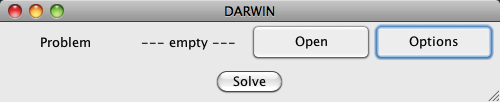
\includegraphics[scale=0.7]{img/manual/01_main_screen}
  \caption{The main screen of DARWIN}
  \label{manual_01_main}
\end{figure}

A set of problems (the ones with uncertain values) is included with the
distribution.

\subsection*{Solving exemplary problems}

DARWIN offers an intuitive and easy to use interface for solving MMO
problems. The main window is presented in Figure~\ref{manual_01_main}. To
solve a~problem one need to execute following steps:

\begin{enumerate}
\item Click the ``Open'' button in the main window.
\item Choose a problem file using a~provided file selector
  (fig.~\ref{manual_02_problem_selector}). The problem has to be described in
  the DARWIN .mod (model) file format.
\item The main window now shows a name of the problem
  (fig.~\ref{manual_03_selected}). Click ``Solve''.
\item A window presenting generated solutions appears
  (fig.~\ref{manual_04_mark_as_good}). Mark preferred solutions as ``good''
  using checkboxes in the ``is good'' column.
\item A window with solution details can be invoked by selecting a~solution
  and clicking the ``Solution details'' button (fig.~\ref{manual_05_dec_var}).
\item After selecting the solutions an evolutionary optimization begins
  (fig.~\ref{manual_06_evo_loop}). New solutions are generated and one can
  mark ``good'' solutions from a new set again.
\item If generated solutions are satisfactory, then one can stop the
  algorithm by clicking ``Mark as good'' when no solutions are selected
  (fig.~\ref{manual_07_finish}).
\end{enumerate}

\begin{figure}[htb]
  \centering
  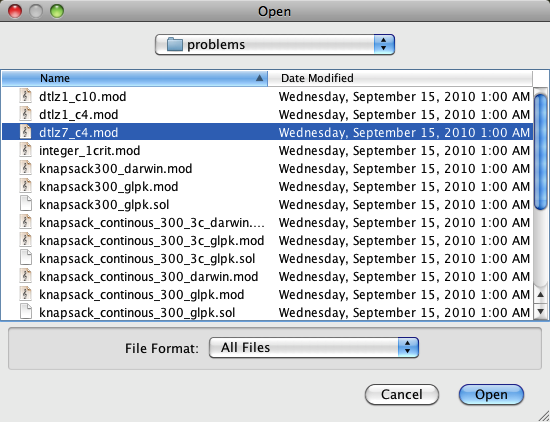
\includegraphics[scale=0.7]{img/manual/02_problem_selector}
  \caption{Selecting a problem to solve}
  \label{manual_02_problem_selector}
\end{figure}

\begin{figure}[htb]
  \centering
  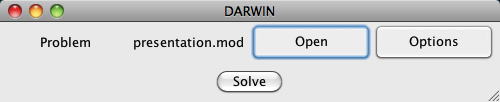
\includegraphics[scale=0.7]{img/manual/03_problem_selected}
  \caption{Starting the algorithm}
  \label{manual_03_selected}
\end{figure}

\begin{figure}
  \centering
  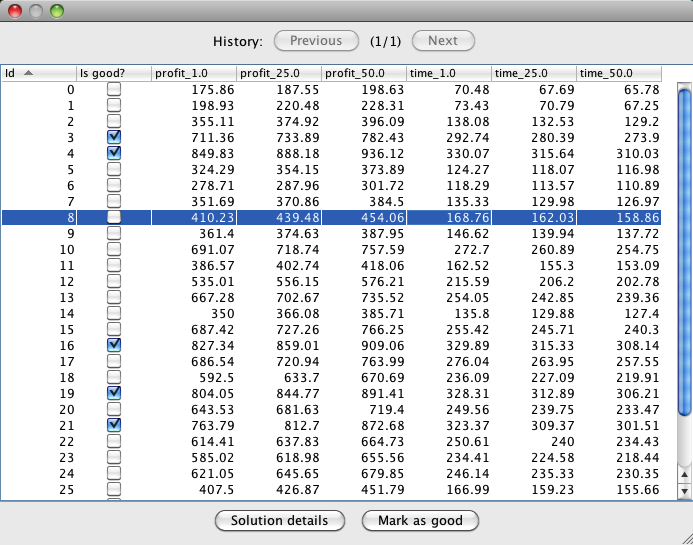
\includegraphics[scale=0.7]{img/manual/04_marking_solutions}
  \caption{Marking the ``good'' subset of generated solutions}
  \label{manual_04_mark_as_good}
\end{figure}

\begin{figure}
  \centering
  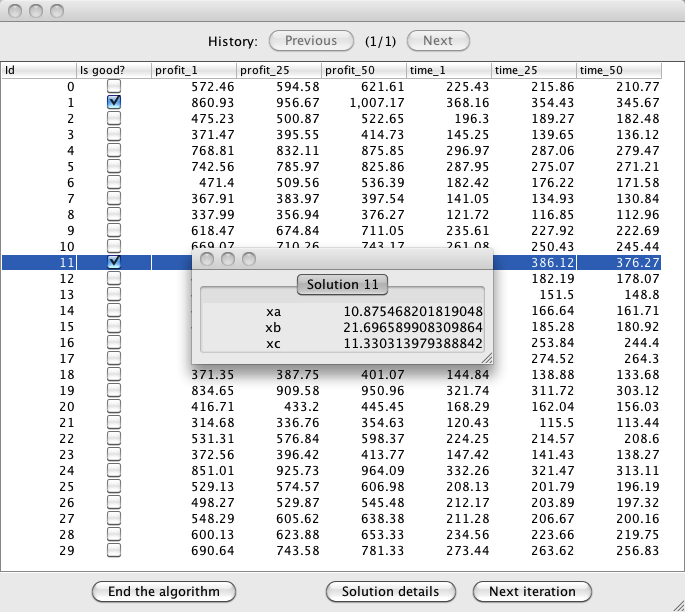
\includegraphics[scale=0.7]{img/manual/05_solution_details}
  \caption{Decision variables for a given solution}
  \label{manual_05_dec_var}
\end{figure}

\begin{figure}
  \centering
  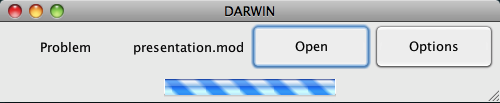
\includegraphics[scale=0.7]{img/manual/06_evolutionary_loop}
  \caption{An evolutionary optimization is performed}
  \label{manual_06_evo_loop}
\end{figure}

\begin{figure}
  \centering
  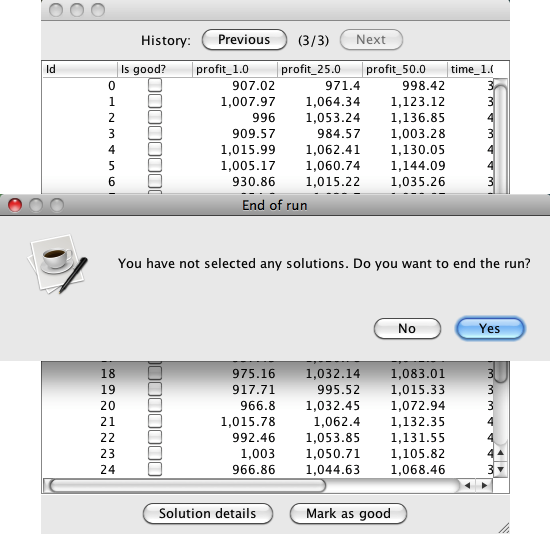
\includegraphics[scale=0.7]{img/manual/07_end_of_run}
  \caption{Finish the problem analysis}
  \label{manual_07_finish}
\end{figure}

\clearpage{}
\subsection*{Advanced options}

The DARWIN GUI offers additional options to customize the process. One can
modify the algorithm parameters in a~configuration dialog
(fig.~\ref{manual_08_options}). To open it, click the ``Options'' button in
the main window. The options are described below.

\begin{table}[htb]
  \centering
  \begin{tabular}{l p{3.5cm} p{6.5cm} l l}
    \hline
    Tab & Option name & Description & Default value \\
    \hline
    \hline
    \multirow{5}{*}{Main}
    & The number of solutions & The number of solutions in a population. & 30 \\
    & The number of scenarios & The number of scenarios on which the solutions will be evaluated.  & 30 \\
    & The number of generations & The number of generations in the interior loop. & 30 \\
    & Percentiles & Which percentiles are meaningful to the decision maker. & 1.0, 25.0, 50.0  \\
    & Use an average in quantiles & Whether an average in quantiles should be used instead of
    the maximum value. & false  \\
    \hline
    \multirow{3}{*}{The Algorithm}
    & Use All Rules instead of DomLem & Should the All Rules algorithm be used
    instead of the default one & false \\
    & The DomLEM confidence level & A level of confidence which the rules generated by the
    DomLem algorithm should at least have. & 0.6 \\
    & Compare using the supposed utility function & If the evolutionary algorithm should use the
    supposed utility instead of a rule-based score. & false \\
    \hline
    \multirow{4}{*}{Fine Tuning} 
    & Delta & The decay of the rule weight (see \ref{idea-algo}). & 0.1  \\
    & Gamma & The coefficient of an elitism. The higher the gamma, the
    higher the probability of choosing a solution with a~higher rank as
    a~parent. & 2.0  \\ 
    & Eta & The initial mutation probability.  & 0.5    \\
    & Omega & The decay rate of the mutation probability. & 0.1  \\
    \hline
    \multirow{5}{*}{Reports} 
    & The reports directory & A directory where reports should be saved. &
    ./reports  \\
    & Save the evolutionary report & If the evolutionary report should be
    saved ia a~file. & false \\
    & Save the decision maker's report & If the DM's report should be
    saved in a~file. & false \\
    & The rules directory & A directory where rules should be saved. &
    ./rules  \\
    & Save rules & If the decision rules generated during a run should be
    saved on a~disk. & false \\
    \hline
    \multirow{1}{*}{GUI Parameters}
    & Digits after a dot & A number of digits that should be displayed after a
    dot. & 2 \\    
    \hline
  \end{tabular}
\end{table}


The window presenting a~list of generated solutions offers additional
features. The list of solutions can be sorted on a given criterion by clicking
the column header (fig.~\ref{manual_09_sorton}). Another useful option is a
history of solutions. The user can review solutions generated in earlier
iterations, return to them and change his or her selections. This is possible
using the history toolbar (see\ref{manual_10_history}).

\begin{figure}
  \centering
  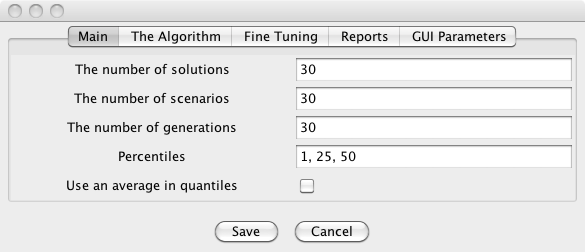
\includegraphics[scale=0.7]{img/manual/08_options}
  \caption{DARWIN configuration options}
  \label{manual_08_options}
\end{figure}

\begin{figure}
  \centering
  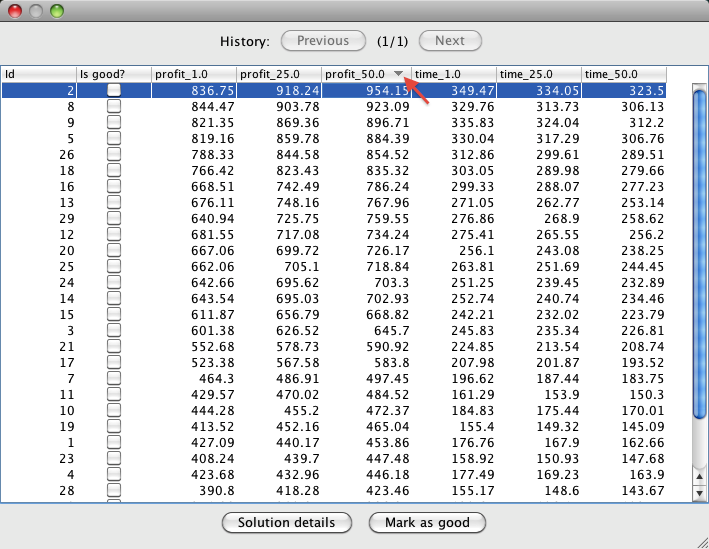
\includegraphics[scale=0.7]{img/manual/09_sorton}
  \caption{Sorting solutions on a given criterion}
  \label{manual_09_sorton}
\end{figure}

\begin{figure}
  \centering
  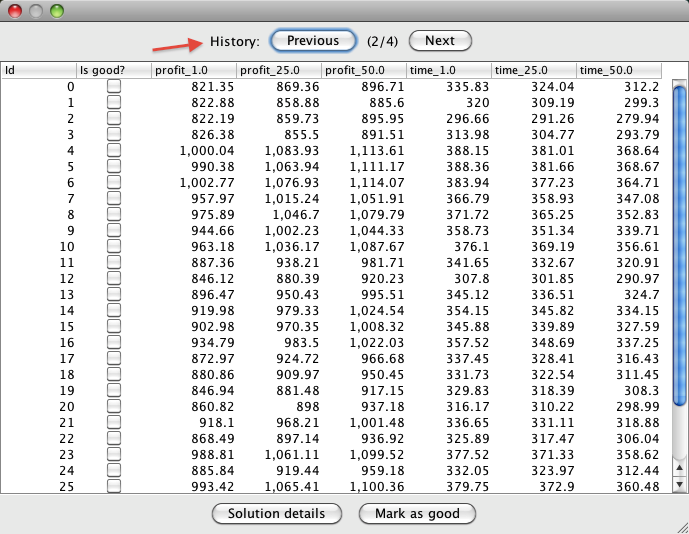
\includegraphics[scale=0.7]{img/manual/10_history}
  \caption{Reviewing the history of generated solutions}
  \label{manual_10_history}
\end{figure}

\clearpage{}
\chapter{The DARWIN .mod file format}

MMO problems for DARWIN are specified in external files. These files are
called the DARWIN model files and usually have the \texttt{.mod}
extension. The application contains a~parser for the model files. The parser
grammar in the Extended Backus-Naur Form (EBNF, see~\cite{Wir77}) is described
below.

\lstinputlisting{res/parser.txt}

Comments handled by a~preprocessor are possible --- (1) line comments,
starting with \texttt{\#}, e.g. \texttt{ \#a-line-comment} and (2) block
comments, enclosed in \texttt{/* */}. Whitespaces are ignored.

A problem file consists of lines, each line contains a~statement ended by
a~semicolon (\texttt{;}). A statement can define the supposed utility
function, a~variable, a~goal or a~constraint. The variables are defining the
problem domain. They can be continuous (with double floating point precision),
binary (indicated by a \texttt{(B)} flag) or integer (\texttt{(I)} flag).
Upper and lower limits of the variable value have to be provided. Each
variable has a name and can be referred by the name in succeeding
statements. Goals are the optimization criteria to be minimized or
maximized. They are named expressions and therefore can be referred later by
the name. Constraints are named inequalities. The inequality is not strict and
both its sides can be expressions. Finally, the supposed utility function is
an expression prefixed with \texttt{!dec:}. The function is useful only if one
wants to mock the decision maker.

An example file with the mix-problem definition is included below.

\lstinputlisting{res/presentation.mod}

The expressions are utilizing intervals (e.g. \texttt{[pa:20, 24]}) and the
supposed utility function is using meaningful percentiles
(e.g. profit$^{25\%}$: \texttt{<profit, 0.25>}).



\chapter{Compiling DARWIN from the source code}

It is possible to build a DARWIN binary from the source code. It can be done
using command line on Windows, Linux and MacOSX.  Instructions are given
below.

\begin{enumerate}

\item \textbf{Get the source code}. Sources are included in a~disk attached to
  the thesis. Alternatively, most recent version is stored in the git
  repository (see~\cite{Loe09})  and can be cloned by typing a~command:\\
  \texttt{\$ git clone git://github.com/puszczyk/DarwinDS.git}
\item \textbf{Prepare a build tool}. DARWIN uses sbt (see~\cite{sbt10})---
  a~build tool for Scala. Detailed setup instructions are given in the
  project's webpage. The easiest way is to install Scala (system-dependent,
  consult \url{http://scala-lang.org} for details) and then prepare a script
  for running sbt. Download sbt-launch.jar from the sbt website:
  \url{http://simple-build-tool.googlecode.com/files/sbt-launch-0.7.4.jar}
  \\
  Somewhere in the \text{PATH} put a script with the following content: \\
  \texttt{java -Xmx512M -jar `dirname \$0`/sbt-launch.jar "\$@"} \\
  or (in case of Windows operating system): \\
  \texttt{set SCRIPT\_DIR=\%~dp0} \\
  \texttt{java -Xmx512M -jar "\%SCRIPT\_DIR\%sbt-launch.jar" \%*} \\
  Make the file executable. It is assumed further, that the script is named
  \texttt{sbt}.
\item \textbf{Build the DARWIN binaries}. Source code is located in the
  \texttt{Darwin} directory. First get required dependencies: \\
  \texttt{\$ cd DarwinDS/Darwin} \\
  \texttt{\$ sbt} \\
  \texttt{> download-jars} \\
  Then run a set of unit-test to check if everything went fine up to this
  point:\\
  \texttt{> test} \\
  This should end with a~message: \\
  \texttt{[info] All tests PASSED.} \\
  \texttt{[success] Successful.} \\
  Now DARWIN can be compiled: \\
  \texttt{> compile} \\
  And run: \\
  \texttt{> run} \\
  To create a \texttt{.jar} package type: \\
  \texttt{> package} \\
  This will generate DARWIN binaries in a subdirectory named \texttt{target}.
\end{enumerate}


\section*{The experiment framework} 

Instead of a graphical user interface, DARWIN can be run in a~console-based
batch mode. This is useful for running a~set of experiments. The batch run can
be invoked by the experiment framework located in the \texttt{Experiment}
directory. The directory contains a few useful scripts written in Bash and
Python. As such it requirers MacOSX or a Linux distribution or a Windows
operating system with Cygwin installed (see~\cite{Laz00}). The utility scripts
are described below:

\begin{itemize}
\item \texttt{runTestPlan.py} --- a script for running a~set of tests. As an
  input it requires a location of the DARWIN directory, a~problem file,
  a~darwin configuration file and a~test plan specification. The problem file
  is a file in the DARWIN .mod file format. The configuration is an .ini file
  structured as follows:
  \begin{lstlisting}
    [section]
    option1 = value1
    option2 = value2
    (...)
    optionN = valueN
  \end{lstlisting}

  
  Required sections and options are described in Table~\ref{t:params}. The
  test plan specification is a text file with the~following structure:
  \begin{lstlisting}
    >test_name_1/number-of-runs
    [section-to-override]
    option-to-override1 = value1
    (...)
    >test_name_N/number-of-runs
    (...)
  \end{lstlisting}

  Each test is run \texttt{number-of-runs} times. For each test one can
  specify a~list of options to be overridden. It is useful for testing an
  influence of a parameter. An example test plan is presented below.
  \begin{lstlisting}
    >delta005/15
    [main]
    delta = 0.05

    >delta015/15
    [main]
    delta = 0.15

    >delta020/15
    [main]
    delta = 0.20

    >delta040/15
    [main]
    delta = 0.40
  \end{lstlisting}

  This plan will run DARWIN fifteen times for each \texttt{delta} value. Run
  reports are saved in a~directory named after the current date and time. Test
  names are the names of subdirectories.

\item \texttt{genCharts.sh} --- a script for charting run reports. It requires
  installing the \texttt{R} environment (see~\cite{kee10}) with
  \texttt{ggplot2} and \texttt{reshape} libraries. The charts to be generated
  are included in the
  \texttt{Chart} directory of the DARWIN distribution. The usage is: \\
  \texttt{\$ genCharts.sh --brief/--full criteria-no best-val charts-dir
    testplan-out-dir} \\
  \texttt{--brief/--full} decides whether all charts or only the overview
  chart should be generated. \texttt{criteria-no} is the~number of criteria in
  the problem. \texttt{best-val} --- an optimal value of the problem, if can
  not be given should be set to $0$. \texttt{charts-dir} is the directory with
  the \texttt{R} charts to be generated. Finally, \texttt{testplan-out-dir} is
  an output directory of the \texttt{runTestPlan.py} script. Available types
  of charts are presented in Figure~\ref{chart_examples}.

  The script will generate distinct charts for each test run. If one wants a
  comparison between the tests, then \texttt{./genSummaryChart.sh} should be
  used instead.

\item \texttt{genSummaryChart.sh} --- a script for charting a comparison
  between different test runs. The usage is similar to \texttt{genCharts.sh},
  however the number of criteria can be omitted, because is irrelevant to the
  task. The usage is: \\
  \texttt{\$ ./genSummaryChart.sh best-val charts-dir testplan-out-dir
    problem-name}\\
  Available types of charts are presented in Figure~\ref{chart_examples2}.



\end{itemize}


%%% Local Variables: 
%%% mode: latex
%%% TeX-master: "main"
%%% End: 



\end{document}